
\documentclass[a4paper,11pt]{article}
\usepackage[a4paper, margin=8em]{geometry}

% usa i pacchetti per la scrittura in italiano
\usepackage[french,italian]{babel}
\usepackage[T1]{fontenc}
\usepackage[utf8]{inputenc}
\frenchspacing 

% usa i pacchetti per la formattazione matematica
\usepackage{amsmath, amssymb, amsthm, amsfonts}

% usa altri pacchetti
\usepackage{gensymb}
\usepackage{hyperref}
\usepackage{standalone}

% imposta il titolo
\title{Appunti Comunicazioni Numeriche}
\author{Luca Seggiani}
\date{2026}

% imposta lo stile
% usa helvetica
\usepackage[scaled]{helvet}
% usa palatino
\usepackage{palatino}
% usa un font monospazio guardabile
\usepackage{lmodern}

\renewcommand{\rmdefault}{ppl}
\renewcommand{\sfdefault}{phv}
\renewcommand{\ttdefault}{lmtt}

% disponi il titolo
\makeatletter
\renewcommand{\maketitle} {
	\begin{center} 
		\begin{minipage}[t]{.8\textwidth}
			\textsf{\huge\bfseries \@title} 
		\end{minipage}%
		\begin{minipage}[t]{.2\textwidth}
			\raggedleft \vspace{-1.65em}
			\textsf{\small \@author} \vfill
			\textsf{\small \@date}
		\end{minipage}
		\par
	\end{center}

	\thispagestyle{empty}
	\pagestyle{fancy}
}
\makeatother

% disponi teoremi
\usepackage{tcolorbox}
\newtcolorbox[auto counter, number within=section]{theorem}[2][]{%
	colback=blue!10, 
	colframe=blue!40!black, 
	sharp corners=northwest,
	fonttitle=\sffamily\bfseries, 
	title=~\thetcbcounter: #2, 
	#1
}

% disponi definizioni
\newtcolorbox[auto counter, number within=section]{definition}[2][]{%
	colback=red!10,
	colframe=red!40!black,
	sharp corners=northwest,
	fonttitle=\sffamily\bfseries,
	title=~\thetcbcounter: #2,
	#1
}

% U.D.M
\newcommand{\amp}{\ensuremath{\mathrm{A}}}
\newcommand{\volt}{\ensuremath{\mathrm{V}}}
\newcommand{\meter}{\ensuremath{\mathrm{m}}}
\newcommand{\second}{\ensuremath{\mathrm{s}}}
\newcommand{\farad}{\ensuremath{\mathrm{F}}}
\newcommand{\henry}{\ensuremath{\mathrm{H}}}
\newcommand{\siemens}{\ensuremath{\mathrm{S}}}

% circuiti
\usepackage{circuitikz}
\usetikzlibrary{babel}

% disegni
\usepackage{pgfplots}
\pgfplotsset{width=10cm,compat=1.9}

% disponi codice
\usepackage{listings}
\usepackage[table]{xcolor}

\lstdefinestyle{codestyle}{
		backgroundcolor=\color{black!5}, 
		commentstyle=\color{codegreen},
		keywordstyle=\bfseries\color{magenta},
		numberstyle=\sffamily\tiny\color{black!60},
		stringstyle=\color{green!50!black},
		basicstyle=\ttfamily\footnotesize,
		breakatwhitespace=false,         
		breaklines=true,                 
		captionpos=b,                    
		keepspaces=true,                 
		numbers=left,                    
		numbersep=5pt,                  
		showspaces=false,                
		showstringspaces=false,
		showtabs=false,                  
		tabsize=2
}

\lstdefinestyle{shellstyle}{
		backgroundcolor=\color{black!5}, 
		basicstyle=\ttfamily\footnotesize\color{black}, 
		commentstyle=\color{black}, 
		keywordstyle=\color{black},
		numberstyle=\color{black!5},
		stringstyle=\color{black}, 
		showspaces=false,
		showstringspaces=false, 
		showtabs=false, 
		tabsize=2, 
		numbers=none, 
		breaklines=true
}

\lstdefinelanguage{javascript}{
	keywords={typeof, new, true, false, catch, function, return, null, catch, switch, var, if, in, while, do, else, case, break},
	keywordstyle=\color{blue}\bfseries,
	ndkeywords={class, export, boolean, throw, implements, import, this},
	ndkeywordstyle=\color{darkgray}\bfseries,
	identifierstyle=\color{black},
	sensitive=false,
	comment=[l]{//},
	morecomment=[s]{/*}{*/},
	commentstyle=\color{purple}\ttfamily,
	stringstyle=\color{red}\ttfamily,
	morestring=[b]',
	morestring=[b]"
}

% disponi sezioni
\usepackage{titlesec}

\titleformat{\section}
	{\sffamily\Large\bfseries} 
	{\thesection}{1em}{} 
\titleformat{\subsection}
	{\sffamily\large\bfseries}   
	{\thesubsection}{1em}{} 
\titleformat{\subsubsection}
	{\sffamily\normalsize\bfseries} 
	{\thesubsubsection}{1em}{}

% disponi alberi
\usepackage{forest}

\forestset{
	rectstyle/.style={
		for tree={rectangle,draw,font=\large\sffamily}
	},
	roundstyle/.style={
		for tree={circle,draw,font=\large}
	}
}

% disponi algoritmi
\usepackage{algorithm}
\usepackage{algorithmic}
\makeatletter
\renewcommand{\ALG@name}{Algoritmo}
\makeatother

% disponi numeri di pagina
\usepackage{fancyhdr}
\fancyhf{} 
\fancyfoot[L]{\sffamily{\thepage}}

\makeatletter
\fancyhead[L]{\raisebox{1ex}[0pt][0pt]{\sffamily{\@title \ \@date}}} 
\fancyhead[R]{\raisebox{1ex}[0pt][0pt]{\sffamily{\@author}}}
\makeatother

\begin{document}
% sezione (data)
\section{Lezione del 21-04-26}

% stili pagina
\thispagestyle{empty}
\pagestyle{fancy}

% testo
Due lezioni fa abbiamo visto le problematiche date dal campionamento e quindi dalla ricostruzione dei segnali. Le problematiche che avevamo introdotto erano in particolare:
\begin{itemize}
	\item La \textit{frequenza minima} di campionamento per non perdere informazione;
	\item L'\textit{interpolatore ideale} per la ricostruzione del segnale a partire dai campioni.
\end{itemize}

\subsection{Interpolazione di campioni}
Iniziamo a vedere alcune tipologie di \textbf{interpolatori}, per soddisfare il secondo quesito fra quelli appena sollevati. 

\subsubsection{Interpolatore a mantenimento}
Ipotizziamo di usare un interpolatore con risposta impulsiva $\mathrm{rect}$, cioè:
$$
p(t) = \mathrm{rect} \left( \frac{t - \frac{T}{2}}{T} \right) \rightarrow P(f) = T \mathrm{sinc}(f T)
$$

Questo interpolatore viene detto \textbf{a mantenimento}. La forma del segnale ricostruito sarà chiaramente una "scalinata" di $\mathrm{rect}$:
$$
\hat{x} (t) = \sum_n x[n] p(t - nT) = \sum_n x[n] \mathrm{rect} \left( \frac{t - \frac{T}{2} - nT}{T} \right)
$$

\begin{center}
	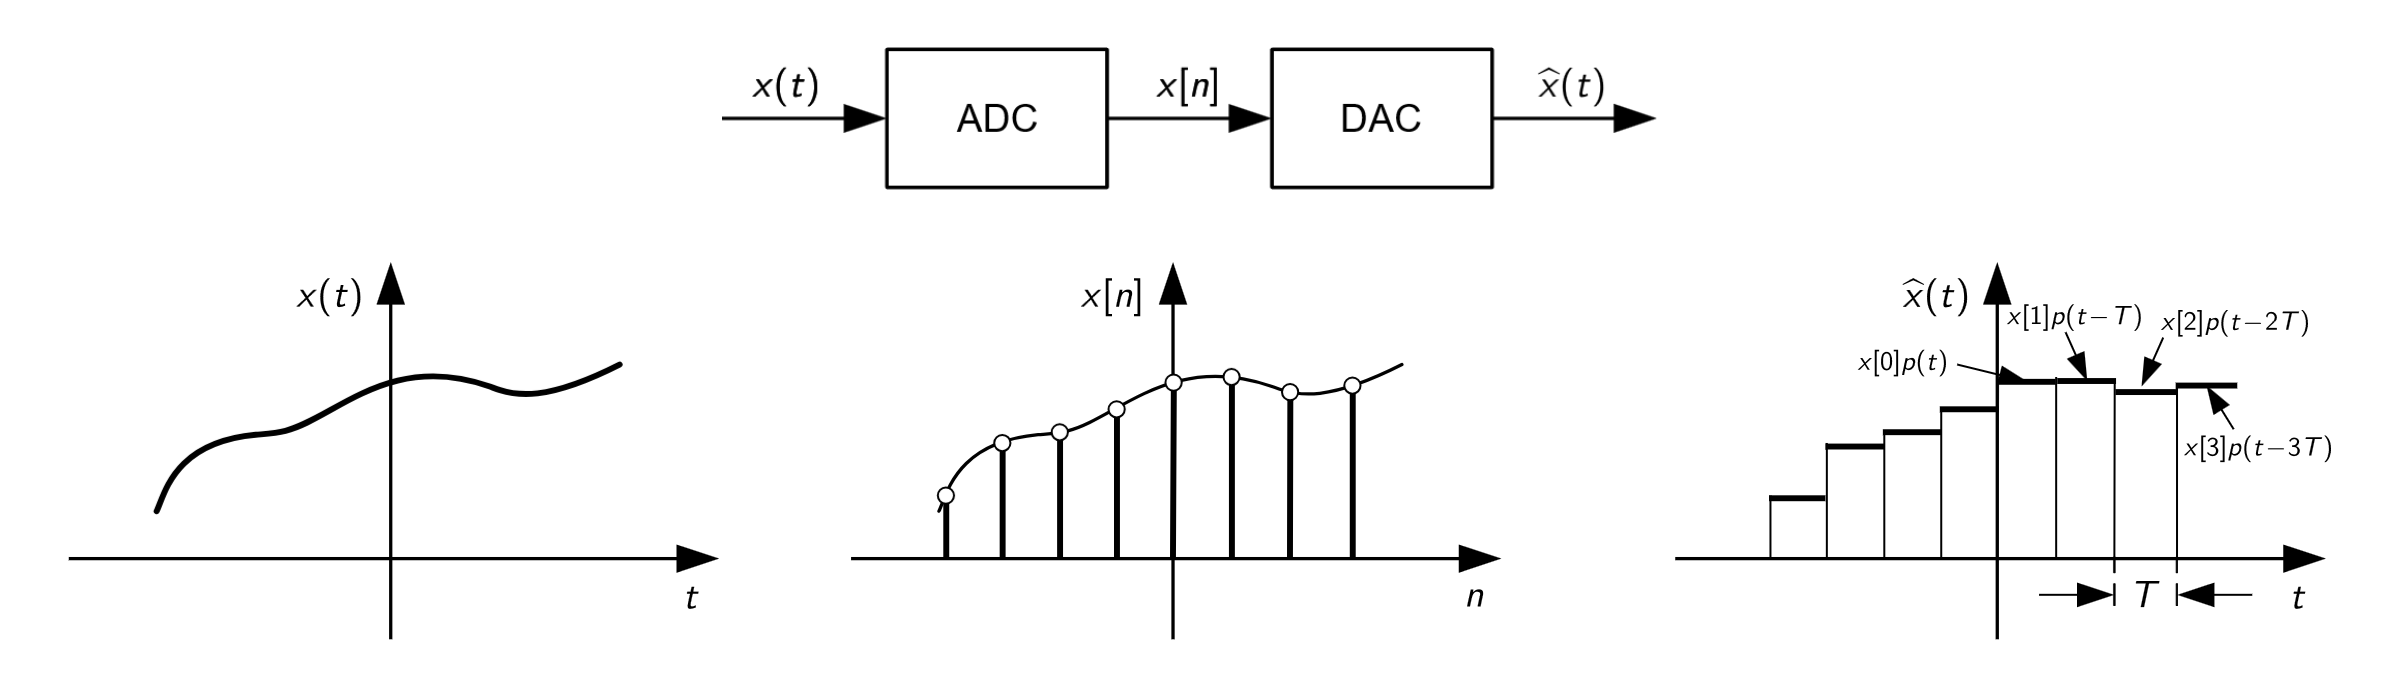
\includegraphics[scale=0.18]{../figures/hold_samp.png}
\end{center}

\par\smallskip

Vediamo quindi la forma della \textit{trasformata} del segnale campionato. Questa sarà semplicemente data dalla sommatoria delle trasformate, cioè delle sinc:
$$
\hat{X}(f) = \sum_n x(nT) P(f) e^{-j2 \pi f n T}
= \sum_n x(nT) e^{-j2 \pi f n T} P(f) = \bar{X}(f) P(f)
$$
Vediamo che tale sommatoria equivale al prodotto fra la trasformata discreta e la risposta in frequenza del filtro a mantenimento ($P(f)$), che altro non sarà che la funzione $\mathrm{sinc}$. 

\begin{center}
	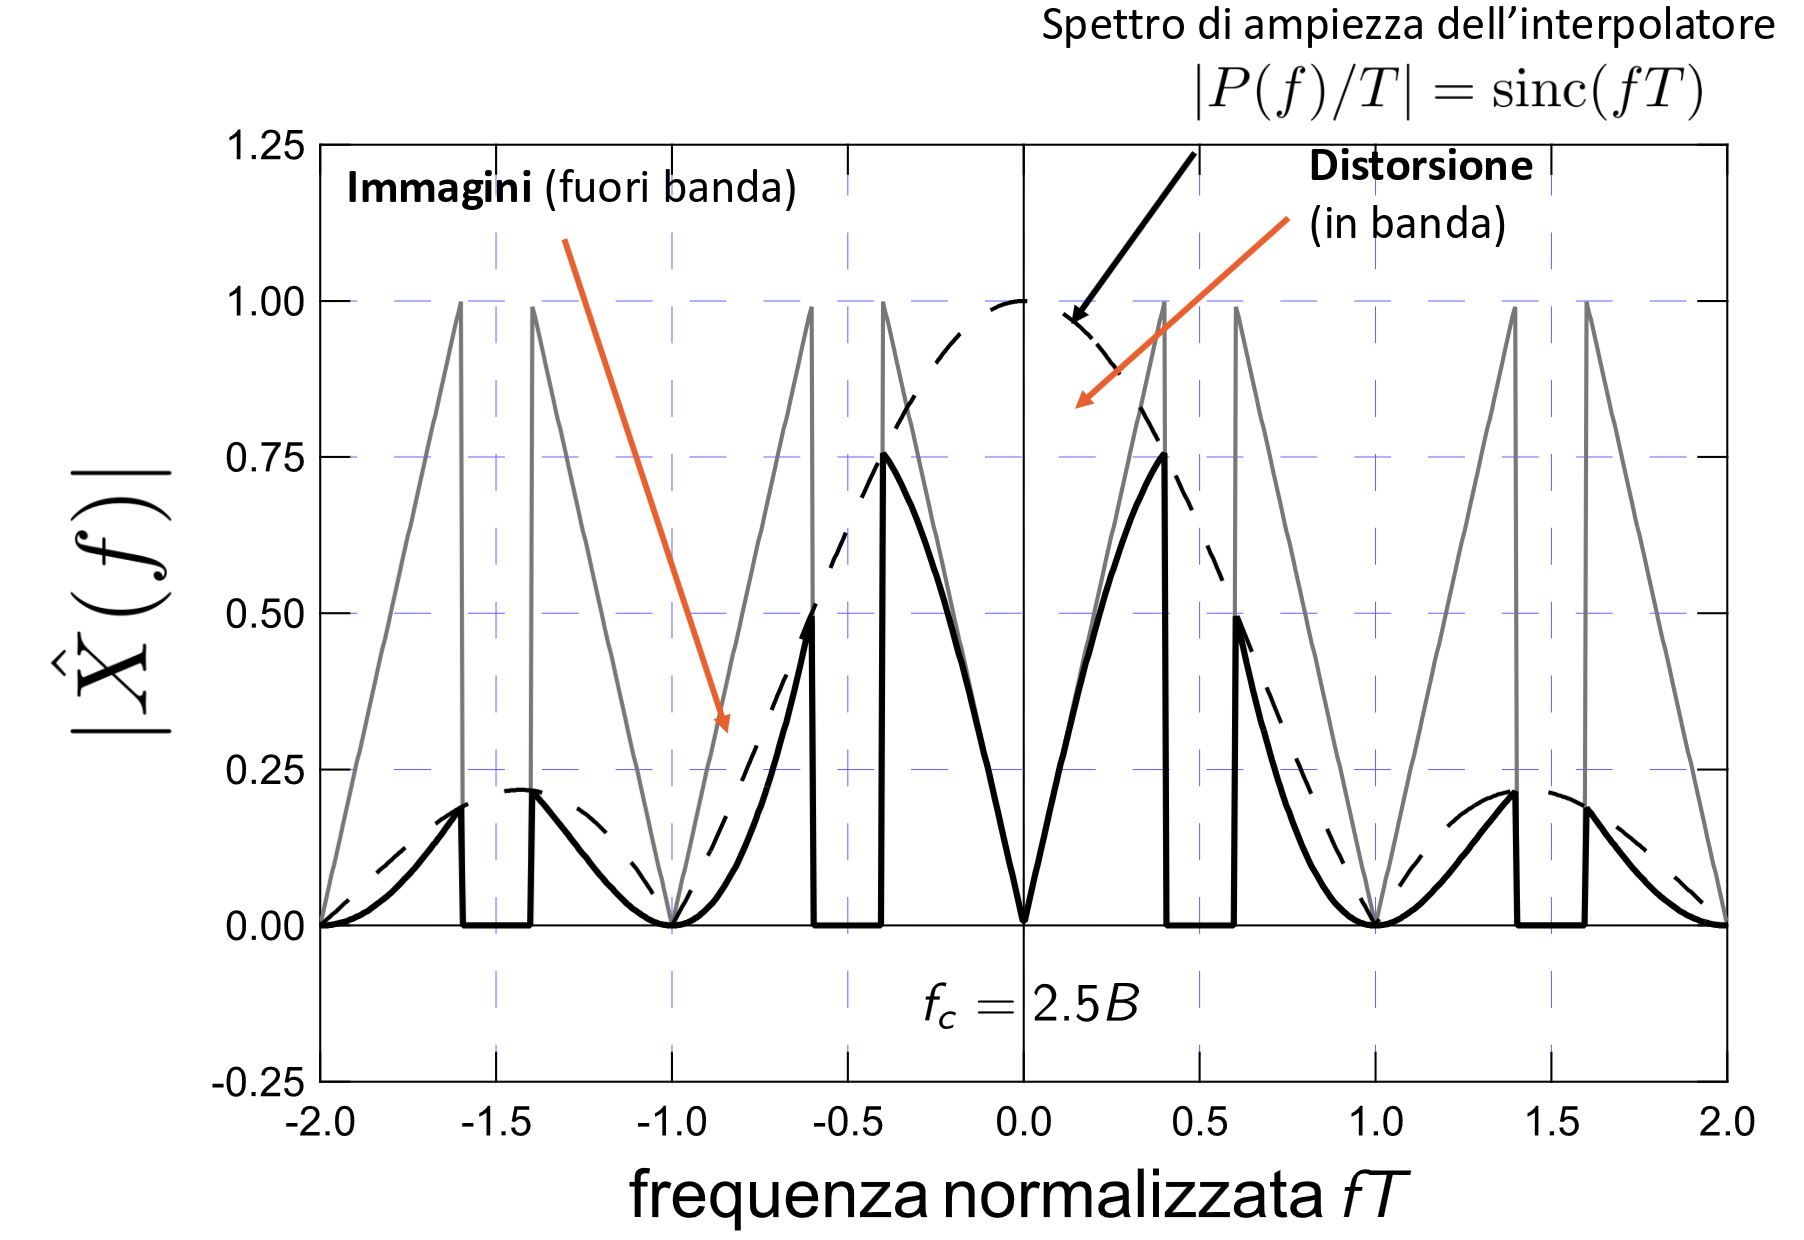
\includegraphics[scale=0.18]{../figures/hold_band.png}
\end{center}

Avremo quindi ridotto lo spettro al suo prodotto con la funzione $\mathrm{sinc}$, quindi limitandone la banda a quella della $\mathrm{sinc}$ stessa. Inoltre ricordiamo che la risposta della $\mathrm{sinc}$ non è lineare attorno alla frequenza $f_0 = 0$, per cui abbiamo una distorsione delle informazioni in banda. Come ultimo dettaglio, notiamo che la $\mathrm{sinc}$ non decade mai a 0, per cui fuori dalla banda di interesse ci troviamo a campionare anche le immagini del segnale date dall'aliasing.

\begin{center}
	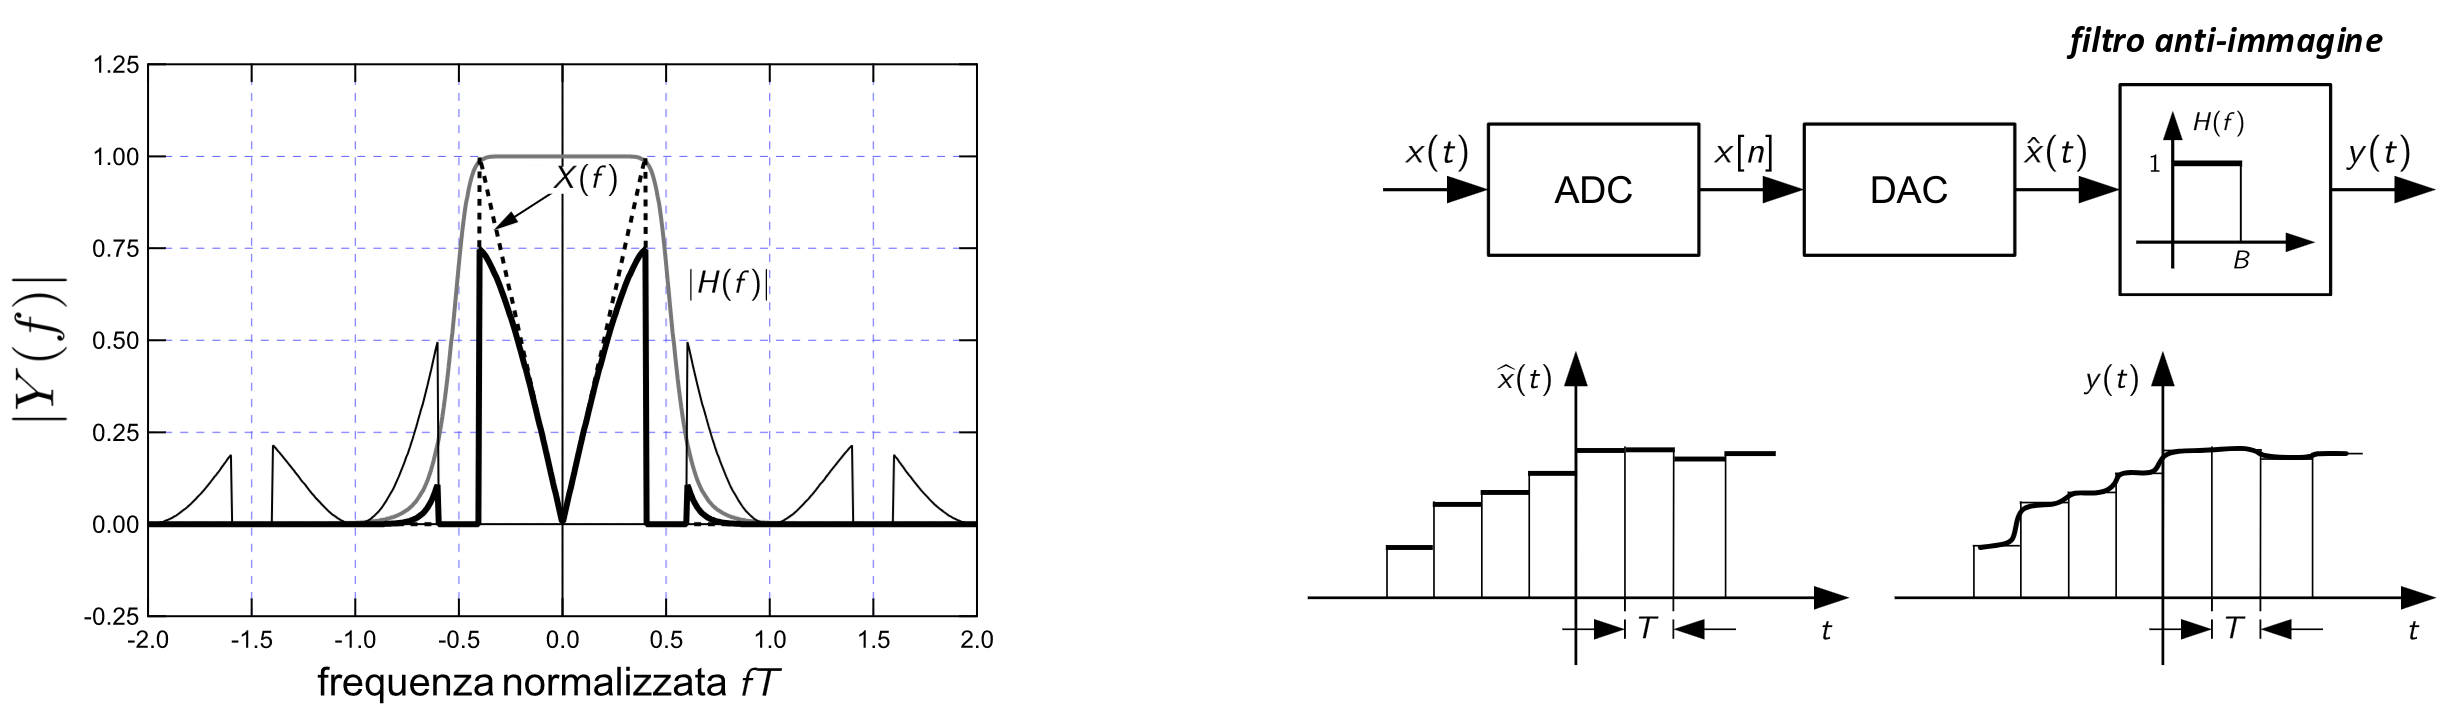
\includegraphics[scale=0.18]{../figures/hold_filt.png}
\end{center}

Proprio per quest'ultimo motivo solitamente i campionatori a mantenimento sono seguiti da filtri passa-basso analogici in uscita (ad esempio semplici filtri RC). Questi effettuano la rimozione delle componenti fuori banda che non ci interessano, e che erano solo distorsione del segnale originale.

\subsubsection{Interpolatore lineare} 
L'alternativa che potremmo considerare è quella dell'interpolatore \textbf{lineare}. La sua risposta impulsiva sarà data dalla $\mathrm{tri}$, cioè:
$$
p(t) = \mathrm{tri} \left( \frac{t - \frac{T}{2}}{T} \right) \rightarrow P(f) = T \mathrm{sinc}^2(f T)
$$

Il fatto che la risposta in frequenza della $\mathrm{tri}$ è la $\mathrm{sinc}^2$ implica che le limitazioni di questo tipo di interpolatore sono le stesse dell'interpolatore a mantenimento, se non con la differenza che la $\mathrm{sinc}^2$ decade più velocemente verso l'infinito, quindi riducendo il numero di componenti fuori banda incluse nel segnale. 

\begin{center}
	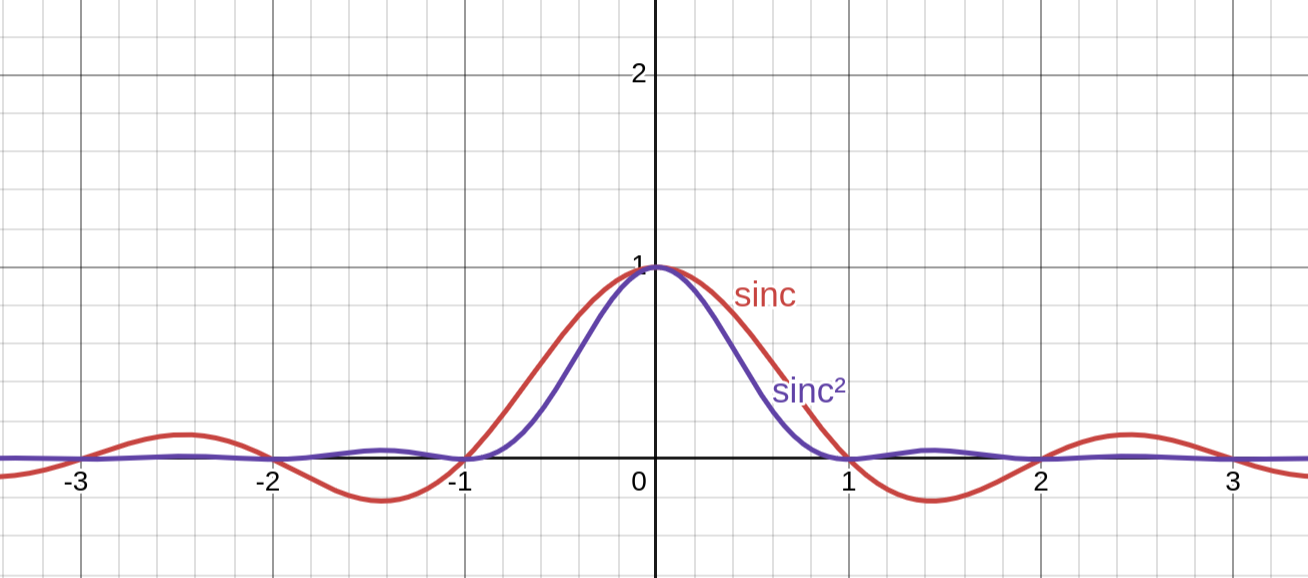
\includegraphics[scale=0.3]{../figures/sinc_vs_sinc2.png}
\end{center}

\subsubsection{Interpolatore cardinale}
Il prossimo interpolatore che vediamo (e quello effettivamente corretto da usare) è l'\textbf{interpolatore cardinale}, cioè quello basato sulla funzione $\mathrm{sinc}$:
$$
P(f) = T \mathrm{rect}(fT) \leftarrow p(t) = \mathrm{sinc}\left( \frac{t}{T} \right)
$$

La forma del segnale a questo punto sarà quella di una sommatoria di $\mathrm{sinc}$:
$$
\hat{x} (t) = \sum_n x[n] \mathrm{sinc} \left( \frac{t - nT}{T} \right) 
$$

Questa sarà chiaramente la soluzione migliore in quanto la risposta in frequenza dell'interpolatore cardinale è una banda pulita e lineare, esattamente corrispondente a quella che ci interessa (fino alla $f_c$ della frequenza di Nyquist). Ricordiamo che avevamo già dimostrato che un segnale limitato in banda a $2B$ viene rappresentato come sommatoria di funzioni $\mathrm{sinc}$ come corollario del teorema 7.4.

\subsubsection{Teorema del campionamento}
Abbiamo, grazie alle osservazioni fatte nelle ultime sezioni, ottenuto un affermazione più concreta del \textbf{teorema del campionamento} di Nyquist-Shannon:

\begin{theorem}{Teorema del campionamento}
Se $x(t)$ è un segnale limitato in banda a $B$ e campionato con frequenza di campionamento $f_c \geq 2B$ (frequenza di Nyquist), allora può essere ricostruito esattamente dai suoi campioni $x[n]$ tramite interpolazione cardinale:
$$
\hat{x} (t) = \sum_n x[n] \mathrm{sinc} \left( \frac{t - nT}{T} \right) = x(t)
$$
\end{theorem}

\subsubsection{Limitazioni dell'interpolatore cardinale}
Il teorema di Nyquist-Shannon ha delle importanti limitazioni che finora non abbiamo considerato (o almeno abbiamo considerato in parte):
\begin{enumerate}
	\item I segnali limitati in banda non esistono in natura: qualsiasi segnale avrà effettivamente una banda infinita (a meno di non essere di durata infinita), che dovremo troncare con un filtro di antialiasing. Abbiamo quindi problemi per quanto riguarda il campionamento alla \textit{frequenza di Nyquist} $f_c = 2B$; 
	\item Risulta impossibile realizzare nella pratica l'interpolatore cardinael, in quanto la funzione $\mathrm{sinc}$ ha componenti $\neq 0$ prima dello 0. Realizzare questo filtro nella realtà significherebbe quindi creare un sistema non causale, che in qualche modo "vede nel futuro". Nemmeno l'\textit{interpolatore cardinale}, quindi, si salva.
\end{enumerate}

Il risultato è che la ricostruzione ideale di segnali secondo il teorema di Nyquist-Shannon è vera nella teoria ma non nella pratica. Dobbiamo sfruttare, nel caso reale, delle approssimazioni.

\par\smallskip

Vediamo come risolvere questi problemi. Per rendere realizzabile la $\mathrm{sinc}$ la cosa migliore che possiamo fare è troncare l'interpolatore cardinale ad una finestra $\mathrm{rect}$ di larghezza $\Delta$:
$$
p_\Delta (t) = \mathrm{sinc} \left( \frac{t}{T} \right) \mathrm{rect} \left( \frac{t}{\Delta} \right)  
$$
A questo punto la formula di ricostruzione del segnale diventa:
$$
\hat{x}(t) = \sum_n x[n] p_\Delta (t - nT)
$$

Ci potremmo interrogare riguardo alla scelta del $\Delta$. In genere. notiamo che conviene scegliere:
$$
\Delta = n T, \quad n \in [10, 200]
$$
cioè multipli naturali dell'intervallo di campionamento $T$, con $n$ intorno al centinaio.

Infine. notiamo che il segnale $p_\Delta(t)$ non è ancora causale, ma solo limitato in durata. Per rendere il sistema effettivamente causale dobbiamo introdurre un ritardo di tempo di $\frac{\Delta}{2}$:
$$
p_\Delta(t - \frac{\Delta}{2})
$$
che riporta la risposta impulsiva nella zona con $t > 0$. Chiaramente a maggior $\Delta$ (quindi migliore approssimazione della $\mathrm{sinc}$) corrisponde un maggiore ritardo.

La formula del segnale diventa a questo punto:
$$
\hat{x} (t) = \sum_n x[n] p_\Delta (t - nT - \frac{\Delta}{2})
$$

\end{document}
